\subsection{Reference resolution}
% SD: Reference resolution task
% DK: (done)
\label{sec:reference_resolution}
\subsubsection*{Setup}
With the reference resolution task, the model is trained to understand referring expressions, by pointing towards the target object in the scene.
Compared to the object identification task in Section \ref{sec:object-identification}, this task is more complex since it also includes identifying locations instead of choosing from given objects.
This level should help to analyze, how the final task of the language game should look like, in especially what the receiver is tasked to predict.
As described before, the sender should communicate an object in the image and the receiver needs to identify it.
The challenge lies in how the receiver refers to the identified object.
There are multiple possibilities, how it can be done.
One of them could be to describe the target object with human language, using the attributes.
The main goal however is to let the language of the agents emerge as natural as possible.
Including human referring expressions into the task would bias also the emerged language towards attributes and words, used in natural language.
For this reason, the final task of the receiver will be to 'point' to the target object.
The models are therefore tasked to predict the center coordinates of the target object.
% SD: Reference resolution with identification of location. The other task, object identification is also resolving reference but it is easier as you are only picking objects. The first task also involves spatial knowledge.
% DK: (done)
With this approach, the models receive few natural language information, but are still able to rely on all information present in the image to discriminate the objects.

To achieve this goal, multiple setups of models are trained.
In the simplest setup, the \textbf{reference resolver}, the model receives only the image as an input and produces two numbers as an output, the predicted x- and y-coordinate of the target object.
% SD: What are the features?
% SD: Note that these are visual features and not spatial features. It is true that visual features also encode some spatial information, how visual features relate to each other, but such information is very different from the spatial information required to predict coordinates in a coordinate frames, and hence we expect the task will be very hard.
% DK: TODO
Again, the image is encoded, using the \emph{image encoder} submodule, described in Section \ref{sec:image-processing}.
The \emph{coordinate predictor} submodule takes the encoder image to predict x- and and y-coordinates of the target image,
Hereby, the encoded image is flattened and passed through two linear layers with a \emph{ReLU} non-linearity in between.
These reduce the dimensions first to the coordinate predictor dimension $c$ and finally to 2.

To determine the loss, the euclidean distance between the resulting predicted point on the image and the ground truth point are calculated.
This distance is learned to be minimized.
By doing that, the model learns to focus and attend on a specific part in the image, in a perfect model the center of the target objects.

With this simple setup, the model is theoretically able to very precisely focus on an object in the image.
% SD: Very precisely. This is higher resolution that attention in the visual models that operates on o 7x7 grid, normally.
% DK: (done)
The problem arises as soon as multiple objects are present in the image.
There is no information available for the model to understand which one of these objects is the actual target object, except for the final calculation of the loss.
Since there is not necessarily a pattern for which object in the image is the correct target object over the whole dataset, the models will likely fail to generalize.
Therefore, the models need to receive more information.
Here, four different ways to encode and refer to the target object are tested.

\begin{figure}[ht]
    \centering
    \subfigure[Model including one-hot encoded attributes and locations]{
        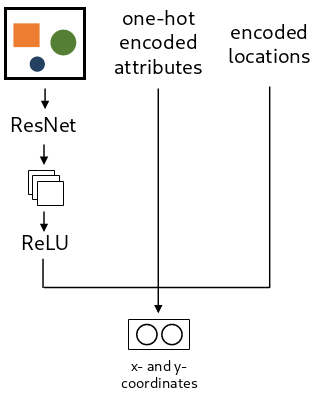
\includegraphics[width=0.35\linewidth]{figures/arch_coordinate_predictor.png}
        \label{fig:coordinate_predictor_architecture}
    }
    \subfigure[Model including incremental referring expression]{
        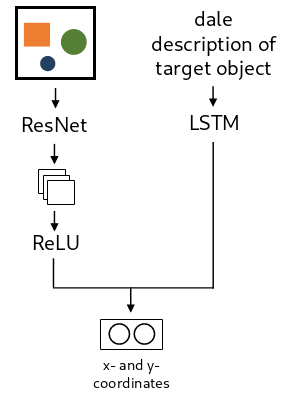
\includegraphics[width=0.34\linewidth]{figures/arch_coordinate_predictor_dale.png}
        \label{fig:coordinate_predictor_dale_architecture}
    }
    \caption{Simplified architecture of the coordinate predictors}
    % SD: How are these encoded?
    % DK: (done)
\end{figure}

In the first method, the target objects' attributes are encoded as \textbf{one-hot encodings}, as described in Section \ref{sec:object-identification}.
In an extension to this method, also the \textbf{center coordinates of all objects} in the image are included.
% SD: Encoded locations?
% DK: (done)
The center coordinates of all objects are simply extracted.
Since there is no direct way of ordering objects, distributed in 2 dimensions into a list, these are shuffled, to just provide the model with all possible targets to choose from.
Since there are varying numbers of objects in the image, this vector of variable length is padded to the maximum number of objects in the dataset.
The padded locations consist of two zeros for both coordinates.
In both methods, the encodings of the target object are concatenated with the encoded image and then passed to the coordinate predictor.
% SD: Why shuffled? If we order them the way they appear in the image, the model will have more information that they are sequentially related.
% DK: (done)
% SD: Convolutions are only applied on visual features, not object attribute features and locations.
% DK: (done)

The third method encodes the attributes of the target object with human language using the \textbf{incremental GRE-algorithm}.
This opposes the idea described before, to share as few natural language information as possible with the model.
Still, this approach can help to understand and analyze if the model was able to extract information about the objects and more specifically their attributes from the image.
% SD: The question you are asking is whether it is possible to predict location from the visual appearance of the object. This is highly complex task as it requires quite two step reasoning, identification of features with that attribute, e.g. blue and then locating that feature in the image.
% DK: TODO
If the model is able to match parts of the image with human words it would show that the model learned this attribute.
If the model in a next step can learn this for the whole dataset, this would mean that it could generalize over these attributes and assign them to certain regions in an image.
This insight would help for succeeding models that make use of these learnings without human language.

% Using the algorithm, one can describe an object using its attributes to discriminate it from other objects as efficiently as possible.
% In other words, the object is described unambiguously using the lowest number of words.
% The algorithm assumes that there is an order of importance for attributes, such as shape, color and size.
% This order defines, which attributes can be left out, while still identifying the object uniquely.
% This research relies on the following order from most important to least important: shape, color, size
% Given for example the scene from \ref{fig:clevr-dale-5} with the target object being the \emph{big purple cylinder}.
% Using all three attributes, this description identifies the object perfectly and uniquely.
% Following the algorithm, we could make the description shorter by removing the least important attribute \emph{size} without loosing unambiguity, describing it as the \emph{purple cylinder}.
% This can be taken even one step further by removing also the \emph{color}.
% Describing it as the \emph{cylinder} still doesn't describe any distractor, since the target object is the only cylinder in the scene.
% % SD: See my point earlier about the reversed algorithm between the two tasks 
% % DK: TODO

For the experiments, each image is captioned with a referring expression of the target object using the described algorithm.
To include it in the model, the referring expressions need to be padded to an equal length.
In this case they are padded to a length of 3, which is the maximum number of attributes that can be used.
For this, as standard practice in captioning tasks, the referring expressions are padded at the end with a specified padding token.

In the model, the referring expression is encoded, using the \emph{GRE parser} submodule.
Here, the learned embeddings of each token are parsed by the LSTM and its final hidden state is then used as a summary of the complete referring expression.
Tokens are embedded with embedding dimensions $LSTM_e$ and the output of the LSTM has the size if $LSTM_o$.
The vocabulary that is used for the descriptions is based on 14 symbols, including the padding token.
Both the processed image and the final hidden state of the LSTM are flattened and concatenated, which is then passed through the coordinate predictor.
% SD: \citep and \citet Use Name (year) when you are referring to particular person and (Name, year) when you are referring to a paper. Hence, in this case it would be the latter.
% DK: done

The fourth method, to encode the target object utilizes \textbf{masking} of the image.
% SD: Oh, before we talked about 3 methods
% DK: done
The image is masked in the same way as in Section \ref{sec:referring_expression_generation}.
While even the one-hot encodings contain human language knowledge by translating human referring descriptions into a vector, the masking method will only point the model towards the target object without giving more information.
It therefore can only rely on its own extracted visual features and the inherent human bias in the image when looking at masked images.
% SD: The information in the masked image is still not enough to identify the precise location, only the region. Hence, it corresponds on attention in the attention models. But those are generating labels and not predicting coordinated. The task is still challenging.
% DK: TODO
Both original and masked image are processed as described in \ref{sec:image-processing} and afterwards passed through the coordinate predictor.

For all setups, the same hyperparameters as in the previous experiments are used: a learning rate of $2\times10^{-4}$, a batch size of 32 samples and 30 epochs, \emph{Adam} \citep{Kingma2015} as optimizer.
8000 randomly selected samples are used for training, the remaining 2000 samples for testing.
The loss is calculated using cross entropy.
Table \ref{tab:variables-reference-resolution} shows the variables that are changed during the experiments for each of the models.

\begin{table}[ht]
    \centering
    \begin{tabular}{lcccc}
        \toprule
                              & $e_i$              & $c$               & $LSTM_e$  & $LSTM_o$               \\
                              & $[100, 500, 1000]$ & $[512,1024,2048]$ & $[15,30]$ & $[500,1000,1500,2000]$ \\\midrule
        reference resolver    & \times             & \times            & -         & -                      \\
        + one-hot             & \times             & \times            & -         & -                      \\
        + one-hot + locations & \times             & \times            & -         & -                      \\
        + incremental RE      & \times             & \times            & \times    & \times                 \\
        + masking             & \times             & \times            & -         & -                      \\
        \bottomrule
    \end{tabular}
    \caption{Variables for each model where $e_i$ is the image embedding dimension, $c$ the dimensions of the coordinate predictor, $LSTM_e$ the embedding dimensions for tokens in the LSTM and $LSTM_o$ the output dimension of the LSTM}
    \label{tab:variables-reference-resolution}
\end{table}

The test dataset is again evaluated on the euclidean distance of the predicted coordinates to the ground truth coordinates.
This distance needs to be minimized.
The mean of all calculated distances is calculated across the whole epoch, which results in a mean distance score per epoch.
Since this score only takes the average of all predictions into account it doesn't show how every prediction fared individually.
If for instance the prediction of one object is getting more precise with growing number of epochs, but the precision of another object gets worse, the mean distance will stay the same.
% SD: Yes that’s correct but through several epochs we hope we will refine the distance and standard deviation of the error. It should level out. It is not a problem. What you do with a circle and accuracy is that you make the task easier as your pointer is now not pointing to a point but to a larger area.
% DK: TODO
It doesn't reflect this change.
For that reason, we also introduced an accuracy score.
For that we defined a fixed size circle with a radius of 20 pixels around the center of each object.
If the model's prediction lies in this circle, it will be counted as a correct prediction, if it lies outside, it is a false prediction.
These scores are averaged for the epoch and result in an accuracy score, where 100\% means that all predictions were very close to the center coordinates and 0\% means that no predictions were close to the center coordinates.
% SD: But here the score will face the same problem with steward deviation. Hence the only difference here is that pointing is less precise.
% DK: TODO
This of course doesn't give a perfect representation since the size of the objects varies, but it will still show, how precise each individual prediction is.
A high accuracy may indicate that the model could identify this specific object better.

The reference resolution models are trained on the 'CLEVR single' as well as on both 'Dale' datasets.
The 'CLEVR single' dataset should test the model if it can actually learn locations of an object.
Since the model relies on the extracted features of either VGG or ResNet, locational information of the objects in the image might not be present anymore.
This is due the fact that CNNs compress information of the image summarizing small regions (convolutions) several times.
While this extracts the key features of objects in an image and might capture relational position between these objects, absolute locations might get lost as shown by \citet{Kelleher2017}.
% SD: Explain. w3 had a paper with John Kelleher on what spatial information is encoded in CNNs
% DK: (done)
Training on this dataset should make sure that the model can converge towards the correct pixels, utilizing these features.
In a next step, the 'Dale' datasets provide the actual problem of discriminating objects from each other and afterwards pointing to the correct one.
Here, the models should make use of the additional given referring expressions about the scene, as one-hot encodings of the attributes, descriptions using the incremental GRE-algorithm or the encoded locations.
'Dale-2' and 'Dale-5' provide two different difficulties for the model, where it needs to discriminate a target object from one or four distractors and then point towards it.
% SD: Point at not just discriminate
% DK: (done)
Latter task is assumed to be significantly harder.

\subsubsection*{Results}

\begin{figure}[ht]
    \centering
    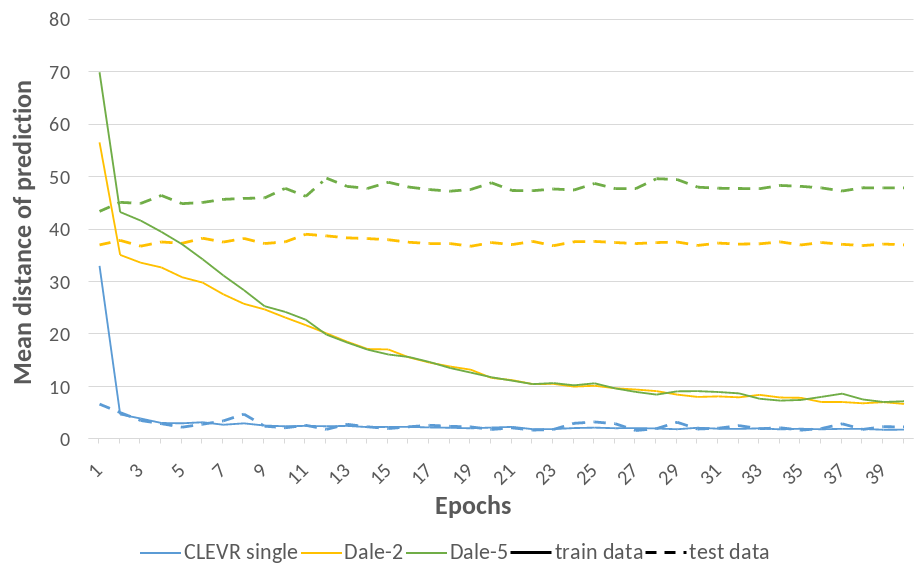
\includegraphics[width=0.8\linewidth]{figures/coordinate-predictor_loss.png}
    \caption{Mean distance between predicted coordinates and ground truth in pixels on different datasets}
    \label{fig:coordinate-predictor_loss}
\end{figure}

Figure \ref{fig:coordinate-predictor_loss} shows the results of the coordinate predictor that doesn't include any information about the target object.
The used feature extractor for these results is \emph{Resnet-3}, but the results don't differ meaningfully from results with other feature extractors.
As can be seen, the success between the different datasets are significant.
The more objects are present in an image, the worse the model performs.
The model converges for the CLEVR single dataset after around 20 epochs to a mean distance of around 2 pixels.
This prediction even though not perfectly on the center point is always on the object.
Opposed to that, using the Dale-2 dataset with two objects, the mean distance lies between 37 and 38 pixels already after the first epoch and doesn't drop with increasing number of epochs.
With five objects in the Dale-5 dataset, the model only predicts a mean distance of around 45 pixels in the beginning, which worsens with a rising number of epochs to 48 pixels.

An interesting observation is the difference of the mean distances between training and testing data.
% SD: How can we have epochs on the testing data? There is no updates so i5 does not make sense.
% DK: TODO
The training distance is constantly approaching zero, while the testing loss is staying constant or even getting higher.
This points to the fact that the model is not generalizing the task by learning abstract patterns that can be applied to unseen data, but is instead memorizing the training data.
That is especially visible for the Dale-5 dataset, where learning the patterns of the training data looses even the ability to interpret some patterns in the testing data.
Applying a higher dropout didn't have an impact on the results.
% SD: The results show that the model is learning something from the training data but this is not the feature that should be learning as the performance on the test data is low. Actually, is it low, it is 10, 35 and 45 pixels. We should not expect any difference between epochs as there is no training. Hence, a flat line is expected.
% DK: TODO

This behavior is indeed not very surprising.
First, results with the 'CLEVR single' dataset show that the model is able to derive geometrical information from abstract feature, extracted by a feature extractor.
Geometrical information therefore doesn't get lost during this abstraction, but the model is able to point to a specific object, as long as only one object is part of the image.
% SD: Because it is in the same location?
% DK: TODO
Secondly, more than one objects present in an image confuses the model, and it is not able to consistently point to one of them.
This can have multiple reasons, for instance that the models lacks the ability to separate objects in the extracted features.
But even in case, the model is able to do that and could determine the location of each object in the scene given the feature, it would not be able to tell, which of these is the actual target object.
The guess is then more or less random.
This especially applies to the Dale-2 dataset, where an identification of the target object just based on one distractor is impossible; both of the present objects are unique.
For the Dale-5 dataset, the model could in theory learn that the target object is always the one object which is unique in respect to its and the distractors' attributes.
This task on the other hand seems very difficult to learn.
In conclusion, the models are able to predict geometrical coordinates, but need more information about the target object to identify it.

When the target object \textbf{attributes are encoded as one-hot vectors} and added to the input, the results don't improve.
One factor that now has a much higher impact is the feature extractor that is used.
Table \ref{tab:feature-extractor-mean-distances} compares the mean distances the models predict for the different feature extractors.
The results are shown for the models trained on the Dale-2 and Dale-5 datasets for training and test data.
First, a big difference can be seen between the datasets.
The models only converge to a minimum mean distance of around 46 pixels to the correct coordinates for the Dale-5 dataset, looking at the test data.
In most cases, it stays above 50 pixels.
% SD: What is the image size? What is the size of a typical object? 50 sounds quite good. Attention is predicting one of 7x7 blocks. Is 50 more or less than 1/7 of an image? 
% DK: TODO
Using the Dale-2 dataset, the behavior is a little different.
All ResNet extractors with four residual blocks and an additional average pooling and optionally a classifier layers reach similar scores as the experiments before without any one-hot encodings.
Interestingly, without the classifier layer, the model doesn't converge at all and the mean distances jump up and down between the epochs.
This effect also applies when using less residual blocks.
Using the VGG, only VGG-cls2 achieve a similar performance, while the others predict coordinates between 43 and 46 pixels away.

\begin{table}[ht]
    \centering
    \begin{tabular}{rcccc}
        \toprule
                            & \multicolumn{2}{c}{\textbf{Dale-2}} & \multicolumn{2}{c}{\textbf{Dale-5}}                                   \\\cmidrule(lr){2-3}\cmidrule(lr){4-5}
                            & train                               & test                                & train          & test           \\\midrule
        \textbf{VGG-0}      & 30,27                               & 46,20                               & \textbf{32,17} & 54,40          \\
        \textbf{VGG-avg}    & \textbf{29,99}                      & 45,08                               & 32,32          & 52,67          \\
        \textbf{VGG-cls1}   & 37,99                               & 43,28                               & 46,57          & 50,75          \\
        \textbf{VGG-cls2}   & 38,87                               & \textbf{39,02}                      & 47,48          & 49,91          \\
        \textbf{VGG-cls3}   & 39,99                               & 44,32                               & 47,26          & \textbf{46,77} \\\midrule
        \textbf{ResNet-3}   & 78,26                               & 65,23                               & 92,07          & 91,12          \\
        \textbf{ResNet-4}   & 44,14                               & 55,24                               & \textbf{36,48} & 58,28          \\
        \textbf{ResNet-avg} & \textbf{33,06}                      & \textbf{39,18}                      & 47,64          & 46,38          \\
        \textbf{ResNet-cls} & 37,57                               & 38,10                               & 44,72          & \textbf{45,92} \\
        \bottomrule
    \end{tabular}
    \caption{Mean test losses for different feature extractors with one-hot attribute encodings after 20 epochs}
    \label{tab:feature-extractor-mean-distances}
    % SD: Explanation of labels
    % DK: TODO
\end{table}

Secondly, the training loss now looks also different.
In almost no cases, the models converge to a lower mean distance than with the test data, meaning a higher precision in their predictions, as they did in the experiment before.
The only exception is ResNet-3 as a feature extractor.
In other words, the models are again not able to generalize, but in specific cases memorize the patterns in the train data.
This hints to the fact that only specific layers of the feature extractors contain information that is generally usable to identify and discriminate objects.
Especially the lower layers with fewer residual blocks in the case of ResNet and no classifier layers for the VGG seem to not encode knowledge that can be utilized for this task.
Higher layers, with more specific encoded information need to be used for this research.
The experiments in the following sections are set up using these higher layers.

Adding \textbf{information about the center coordinates} of all objects should have helped the models to get a list of possible predictions.
In theory, the model could learn to choose between these coordinates by relating them to the extracted features of the image.
This hypothesis doesn't hold.
All results for both datasets Dale-2 and Dale-5 are the exact same as without included information about the locations.
The problem therefore doesn't seem to lie in predicting coordinates in general, but predicting the coordinates of the target object.
% SD: Perhaps arranging the objects sequentially would help the model learn spatial contiguity, see my earlier comment.
% DK: TODO
The model is still not able to understand, which object is the target object.
For that reason, a better representation of the target object is necessary.

In a next step, information about the attributes is included using the \textbf{incremental GRE-algorithm}.
Again, the mean distance of the predictions as well as the accuracy doesn't improve compared to the previous experiments.
% SD: Table with these results?
% DK: the table would show the same figures as the existing table. Should be still included? (QUESTION)

\begin{figure}[ht]
    \centering
    \subfigure['Dale-2', train split]{
        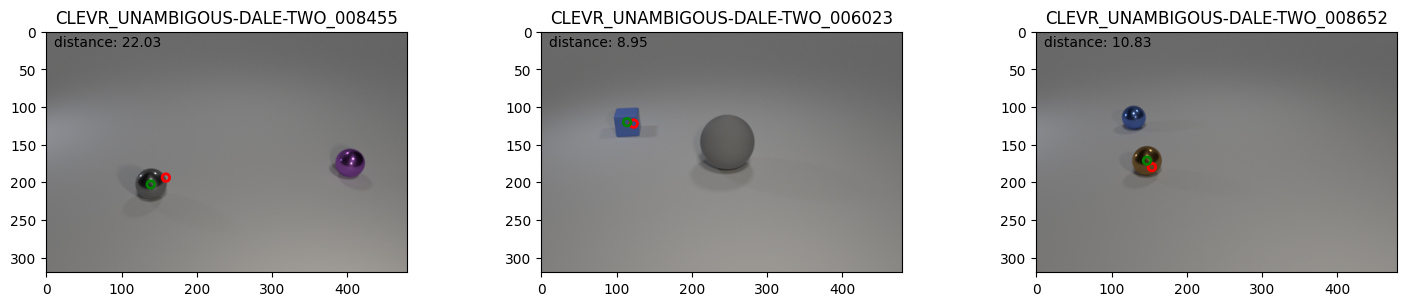
\includegraphics[width=.92\linewidth]{figures/visualization_dale-2_train.png}
        \label{fig:visualizations_dale-2_train}
    }
    \subfigure['Dale-2', test split]{
        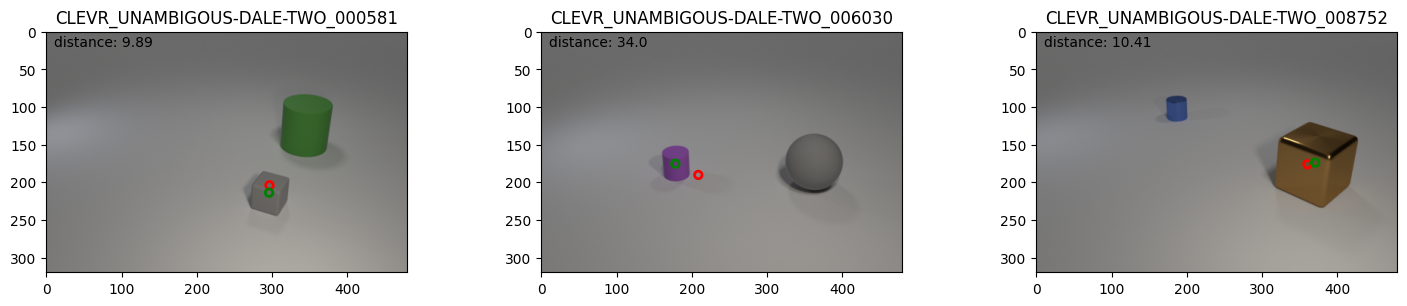
\includegraphics[width=.92\linewidth]{figures/visualization_dale-2_test.png}
        \label{fig:visualizations_dale-2_test}
    }
    \subfigure['Dale-5', train split]{
        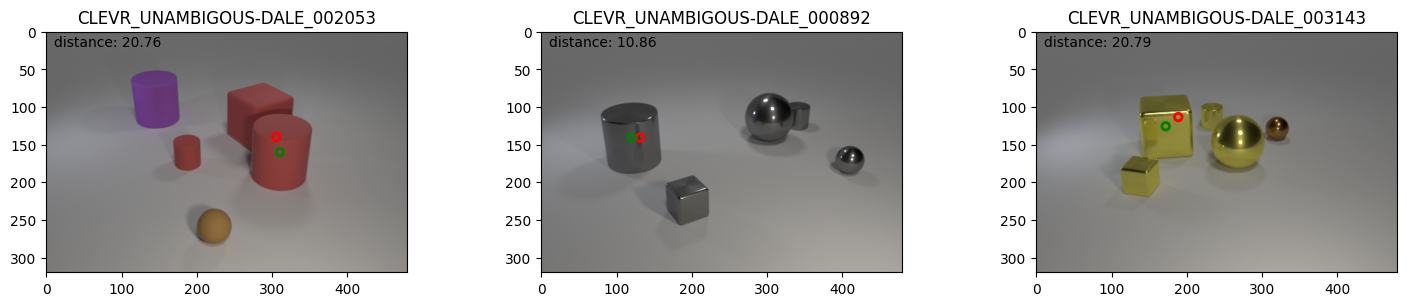
\includegraphics[width=.92\linewidth]{figures/visualization_dale-5_train.png}
        \label{fig:visualizations_dale-5_train}
    }
    \subfigure['Dale-5', test split]{
        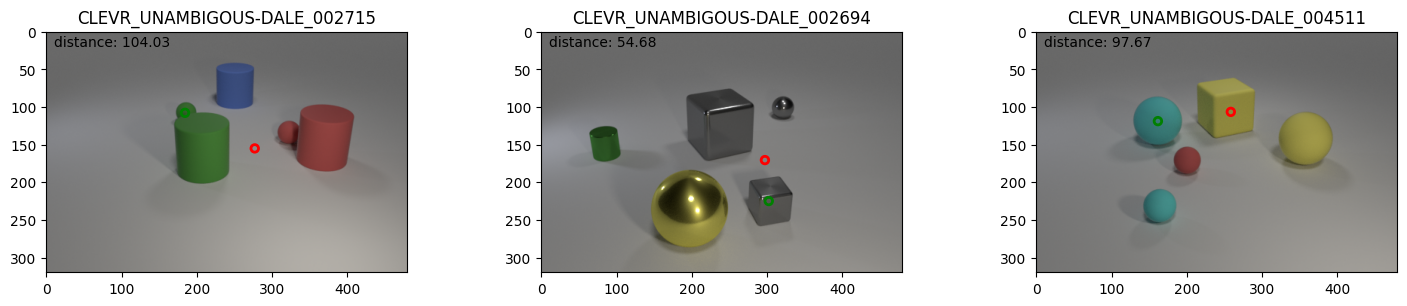
\includegraphics[width=.92\linewidth]{figures/visualization_dale-5_test.png}
        \label{fig:visualizations_dale-5_test}
    }
    \caption{Visualization of the models' predictions in the 'Dale' datasets}
    \label{fig:visualizations_dale}
\end{figure}

An interesting pattern appears when doing a qualitative analysis of the models' predictions.
Here, we visualized the predicted coordinates compared to the ground truth coordinates.
Figure \ref{fig:visualizations_dale-2_train} shows random examples of predictions for images in the train dataset of Dale-2.
The green circle shows the ground truth center coordinates of the target object, while the red circle shows the prediction of the model.
As can be seen, the predictions are very precise.
Figure \ref{fig:visualizations_dale-2_complete_train} combines the predictions and ground truths across all images in the train dataset.
This shows general patterns of the models predictions over the complete dataset.
Here, all predicted coordinates are placed as red circles into the image, while all ground truth coordinates are placed as green circles.
The resulting shape is a rhombus, which reflects that all objects are placed usually central into the scene.
As expected the green and red rhombus align mostly in the same area for the train split of the 'Dale-2' dataset.
% SD: But this image does not show clearly whether the circles for the same object match. You could calculate the average error in distance between the ground truth and predicted coordinates.
% DK: that is done in the quantitative analysis (mean square error above). The visualization should show general learned patterns of the model (as in this case predictions toard the center)

The results look very different for the test split.
As can be seen in Figure \ref{fig:visualizations_dale-2_test}, the three randomly selected predictions don't align with the ground truth coordinates.
For all the images, the predictions don't lie on any object.
In the left image as well as in the central image, the predictions are closer to the target object than towards the distractor, but are still quite imprecise.
% SD: They are closer to the target than distractor and you can see that it is working to a point. But remember this task is very challenging and I wouldn't say the results are so negative.
% DK: right, this is addressed in the conclusions below
These findings align with the mean distance scores, described in the sections before.
However, it seems that the model's predictions are all towards the center of the image.
This can be seen clearer in Figure \ref{fig:visualizations_dale-2_complete_test}.
Again, the green circles form the shape of rhombus.
In contrast, the predictions in red almost all cluster in the center of the image.
They form roughly the shape of a smaller rhombus.
% SD: There is a bias towards the centre but I would not say that the model has not learned anything. I'm surprised that it works so well given the feature representation we have, i.e. no geometric features.
% DK: again, conclusion below
This behavior can be observed for all datasets and architectures of the model.
Figures \ref{fig:visualizations_dale-5_train}, \ref{fig:visualizations_dale-5_test}, \ref{fig:visualizations_dale-5_complete_train} and \ref{fig:visualizations_dale-5_complete_test} show the results for the 'Dale-5' dataset.
Here, the model more likely predicts the center coordinates of a distractor object as seen in the right image, which is also reflected in the lower score of the mean distance.
Also the combined visualization shows the same clustering of predictions in the center of the scene, but the pattern of the smaller rhombus is more visible.
% SD: The centre bias could be the way the error function is used, that is averages all distances and of course this has a tendency to some middle distance. A solution would be to have better geometric features that could take these errors better into account.
% DK: TODO (future work)

\begin{figure}[ht]
    \centering
    \subfigure['Dale-2', train split]{
        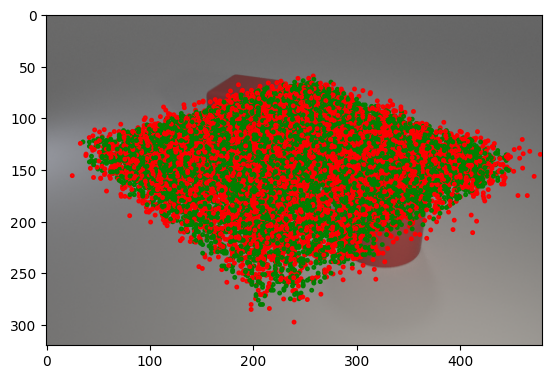
\includegraphics[width=0.42\linewidth]{figures/visualization_dale-2_train_complete.png}
        \label{fig:visualizations_dale-2_complete_train}
    }
    \subfigure['Dale-2', test split]{
        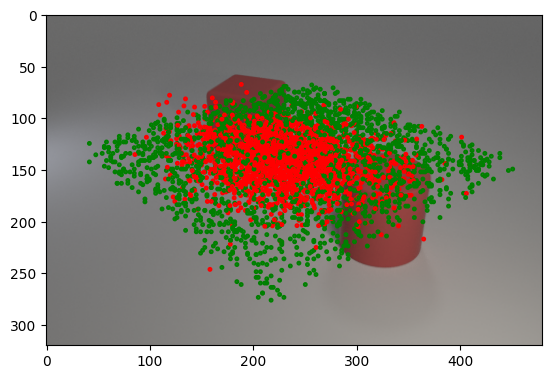
\includegraphics[width=0.42\linewidth]{figures/visualization_dale-2_test_complete.png}
        \label{fig:visualizations_dale-2_complete_test}
    }
    \subfigure['Dale-5', train split]{
        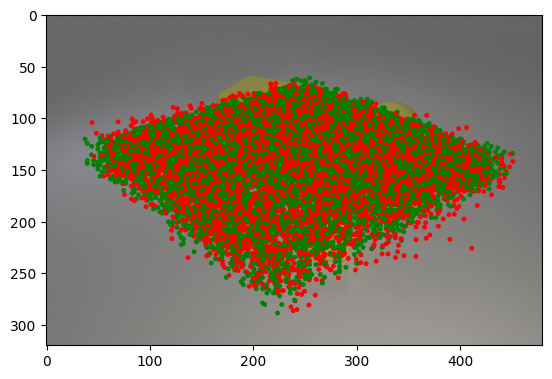
\includegraphics[width=0.42\linewidth]{figures/visualization_dale-5_train_complete.png}
        \label{fig:visualizations_dale-5_complete_train}
    }
    \subfigure['Dale-5', test split]{
        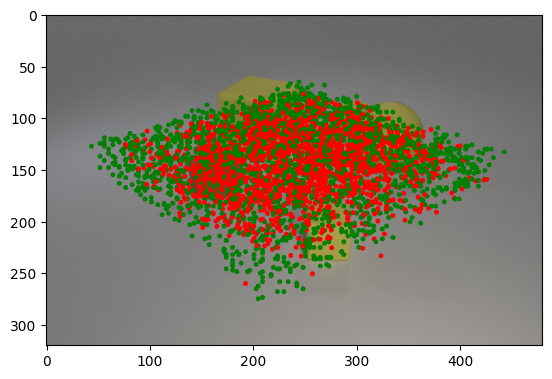
\includegraphics[width=0.42\linewidth]{figures/visualization_dale-5_test_complete.png}
        \label{fig:visualizations_dale-5_complete_test}
    }
    \caption{Visualization of the models' predictions in the Dale datasets}
    % SD: I Haven't checked the earlier captions, but the captions should be informative in the sense that one does not need to look for the text to understand them. Hence, include a brief summary of what each figure contains.
    % DK: TODO
    \label{fig:visualizations_dale_complete}
\end{figure}

These results allow two conclusions.
First, the models are biased to predict coordinates in the center of the image.
% SD: centre - using British English?
% DK: so far I used always American English (hopefully consistently)
The reason for this is likely that the model can produce a relatively low loss, without relying on many extracted features of the objects.
Since all objects are always located in the center of the image and never in its corners, a prediction of any coordinate in the center is on average closer to the target object than any random prediction or predictions of coordinates at the borders of the image.
The model therefore learns only, where any object is likely located and can minimize the mean distance to a certain extent with this strategy.

Second, even though the models are biased towards the center of the image, the predictions are still often leaning towards the location where many objects lie.
This can be seen for the 'Dale-5' dataset, especially in left and central image in Figure \ref{fig:visualizations_dale-5_test}.
Again, by this strategy, the model can minimize the mean distance, since the probability is high that the target object lies in this cluster of objects.
Concluding, the model is able to extract, where objects are located in the image, but can't make use of the referring expressions, to decide which of these objects is the target object.
% SD: There is a centre bias and the model can partially locate the target. The task is hard. The features are not optimal for this task. Future would should focus on using geometric features - we should have tried these and I'm sure we would get better results. Another extension would be making pointing less precise, i.e. focus on a single point, i.e. using a circle of 20 pixels or a 7x7 grid as in the attention mechanism. This would simplify the task.
% DK: TODO (future work)